\documentclass[a4paper]{article}
\usepackage{femape}
\title{Grundlagen der Rechnerarchitektur}
\author{Felix Leitl}
\begin{document}
	\maketitle
	\tableofcontents
	\newpage
	\section{Zahlensysteme}
	\subsection{Präfixe}
		\begin{tabular}{c|c|c|c}
			Kilo & $10^3$ & Kibi & $2^{10}$ \\
			Mega & $10^6$ & Mebi & $2^{20}$ \\
			Giga & $10^9$ & Gibi & $2^{30}$ \\
			Tera & $10^12$ & Tebi & $2^{40}$ \\
			Peta & $10^15$ & Pebi & $2^{50}$
		\end{tabular}
	\subsection{Multiplikation und Division mit Zweierpotenzen}
		Bei Multiplikation einen shift nach links, bei Division einen shift nach rechts:
		\begin{align*}
			0xAB\cdot 2^2=10101011&<<2=1010101100=0x2AC \\
			0xAB/2^2= 10101011&>>2=00101010=0x2A
		\end{align*}
	\section{Rechnerarchitektur}
	\subsection{Endo- vs. Befehlsarchitektur}
		Exteren Sicht(Befehlsarchitektur): Was muss nach außen hin sichtbar sein, damit man den Computer programmieren kann? \newline \newline
		Interne Sicht(Endoarchitektur): Wie werden die Funktionalitäten intern realisiert?
	\subsection{Von-Neumann, URA und ISA}
		7 Eigenschaften des URAs/von-Neumann Architektur:
		\begin{enumerate}
			\item Rechner besteht aus 4 Werken:
				\begin{enumerate}
					\item Rechenwerk
					\item Speicherwerk
					\item Ein-/Ausgabewerk
					\item Leitwerk
				\end{enumerate}
			\item Rechner ist programmgestuerert
			\item Programme und Daten im selben Speicher
			\item Hauptspeicher ist in Zellen gleicher Größe aufgeteilt, jede Zelle hat eine Adresse
			\item Programm ist eine Sequenz an Befehlen
			\item Abweichung von sequentieller Ausführung durch Sprünge möglich
			\item Rechner verwendet Binärdarstellung
		\end{enumerate}
	\subsection{Befehlszyklus}
		von-Neumann-Befehlszyklus:
		\begin{enumerate}
			\item Befehl holen
			\item Befehl dekodieren
			\item Operanden holen
			\item Befehl ausführen
			\item Ergebnis zurückschreiben
			\item Nächsten Befehl addresieren
		\end{enumerate}

	\section{Assemblertheorie}
	\subsection{RiscV-Befehlssatz}
		\begin{center}
			\begin{tabular}{c|ccc|c}
			add[i] & x1 & x2 & x3 \\
			and[i] & x1 & x2 & x3 \\
			or[i] & x1 & x2 & x3 \\
			xor[i] & x1 & x2 & x3 \\
			sll[i] & x1 & x2 & x3 & \text{shift left}\\
			srl[i] & x1 & x2 & x3 & \text{shift right}\\
			mv & x1 & x2 & &\text{move}\\ 
			neg & x1 & x2 & &\text{logical negation}\\
			not & x1 & x2 & &\text{bitwise negation}\\
			sub & x1 & x2 & x3 \\
			mul & x1 & x2 & x3 \\
			div & x1 & x2 & x3 \\
			rem & x1 & x2 & x3 &\text{remainder}\\
			li & x1 & \text{Imm} &\\
			la & x1 & \text{lable} &\\
			lb & x1 & \text{Imm}(x2) & & \text{load byte}\\
			lh & x1 & \text{Imm}(x2) &\\
			lw & x1 & \text{Imm}(x2) &\\
			sb & x1 & \text{Imm}(x2) & &\text{store byte}\\
			sh & x1 & \text{Imm}(x2) &\\
			sw & x1 & \text{Imm}(x2) &\\
			call & \text{lable} & &\\
			ret & & &
			\end{tabular}
		\end{center}
	\subsection{Speicherbereiche}
		\begin{center}
			\begin{tabular}{c|c|c|c|c}
				& & Schreibbar & Ausführbar & Dynamisch wachsend \\
				\hline
				Textsegment & Programmcode & Nein & Ja & Nein \\
				\hline
				Datensegment & Globale Variablen & Ja & Nein & Nein \\
				\hline
				Stack & Lokale Variablen & Ja & Nein & Ja \\
				\hline
				Heap & langlebige Variablen & Ja & Nein & ja
				
			\end{tabular}
		\end{center}
	\subsection{Stack}
		In RiscV wächst der Stack von oben nach unten. RiscV bietet ein spezielles Stackpointer-Register(sp Register), welches immer auf die Adresse des zuletzt hinzugefügten Elements zeigt
		\subsubsection{Lesen vom Stack}
			Letztes Element des Stacks lesen: \verb|lw t0, (sp)| \newline
			Vorletztes Element des Stacks lesen: \verb|lw t0, 4(sp)| (hier ein Integer (word))
		\subsubsection{Schreiben auf den Stack}
			Ein Element auf den Stack legen: \newline
			\verb|li t0, 10|\newline
			\verb|addi sp, sp, -4|\newline
			\verb|sw, t0, (sp)|
			\newline \newline
			Mehrere Elemente auf den Stack legen: \newline
			\verb|addi sp, sp,  -12|\newline
			\verb|sw, t0, 8(sp)|\newline
			\verb|sw, t1, 4(sp)|\newline
			\verb|sw, t2, (sp)|
		\subsection{Speicher freigeben}
			\verb|addi sp, sp, 4|
	\section{Mikroprogrammierung}
		Durch Mikroprogrammierung muss nicht zwangsläufig jeder Befehl fest verdrahtet sein, er kann auch emuliert werden. Besonders bei sehr großen Befehlssätzen (CISC(Complex Instruction Set Computer)) \newline \newline
		\textbf{Mikroprogrammierung} bedeutet, komplexe \textbf{Maschinenbefehle} zur Laufzeit in der CPU durch eine Reihe an noch kleineren, einfacheren Befehlen zu emulieren. \textbf{Assembler-Programme} sind demnach \textbf{Makroprogramme}
	\subsection{Aufbau}
		Ein Mirko-Programm besteht aus aus 4 Kernbestandteilen:
		\begin{itemize}
	  		\item Steuerleitungen
	  		\item ALU (Arithmetisch-logische Einheit)
	  		\item Zwischenregister
	  		\item Tri-State (Schalter zum Öffnen und Schließen der Datenleitungen)
		\end{itemize}
	\subsection{Horizontsal vs. vertikal}
		\subsubsection{Horizontal}
			Für jede Steuerleitung wird ein Bit im Mikrobefehl verwendet. Vorteil, keine Dekodierung. Nachteil, Speicherverschwednung
		\subsubsection{Vertikal}
			Steuerleitungen werden gruppiert, was zu kürzeren Mikrobefehlen führt. Vorteil, speichereffizient. Nachteil, zur Laufzeit muss der komprimierte Befehl wieder in Leitungssignale umgewandelt werden
	\subsection{Beispiel}
		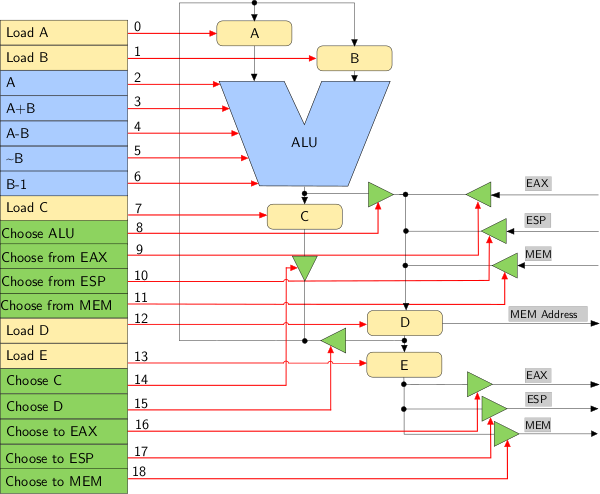
\includegraphics[scale=0.75]{mikroprogrammwerk.png}
		\begin{center}
			\begin{tabular} {|c|c|}
			\hline
			Zeile & Instruktion \\
			\hline
			0 & ESP $\rarr$ B \\
			\hline
			1 & B-1$\rarr$C \\
			\hline
			2 & C$\rarr$B \\
			\hline
			3 & B-1$\rarr$D \\
			\hline
			4 & D$\rarr$ESP \\
			\hline
		\end{tabular}	
		\end{center}
		
				
	
	\section{Befehlssatzarchitektur}
	\subsection{Register-Register}
		Alle Operanden eines Assemblerbefehls müssen in einem Register stehen \newline \newline
		\verb|load R1, A|\newline
		\verb|load R2, B|\newline
		\verb|add R3, R1, R2|\newline
		\verb|store R3, C|
	\subsection{Register-Memory}
		Operanden können sowohl in den Registern, als auch in Speicherzellen liegen
		\newline \newline
		\verb|load R1, A|\newline
		\verb|add R1, B|\newline
		\verb|store R1, C|
	\subsection{Akkumulator}
		Der erste Operand wird mittels load in den Akkumulator geladen, der zweite kommt aus dem Speicher
		\newline \newline
		\verb|load A|\newline
		\verb|add B|\newline
		\verb|store C|
	\subsection{Stack}
		Operanden werden zuerst auf den Stack gepushed. Assemblerbefehle nimmt dann die obersten Werte vom Stack und rechnet damit. Ergebnis landet ebenfalls auf dem Stack
		\newline \newline
		\verb|push A|\newline
		\verb|push B|\newline
		\verb|add|\newline
		\verb|pop C|
	\section{Endianess and Alignment}
	\subsection{Endianess}
		Die Endianess beschreibt, in welcher Reihenfolge die Bytes innerhalb zusammenhängender Datums abgespeichert werden\newline
		\textbf{Little Endian}: Least Significant Byte first \newline
		\textbf{Big Endian}: Most Significant Byte first 
	\subsection{Alignment}
		Um sicherzustellen, dass der Zugriff auf ein Datum möglichst wenig Speicherzugriffe benötigt, ist richtiges Alignment nötig. Ein Datum ist korrekt alignd, wenn gilt: 
		$$
			\text{Adresse(Datum)}\%\text{Größe(Datum)}=0
		$$
		Um Daten korrekt auszurichten muss man unter Umständen Padding einfügen, also freien Platz. \newline \newline
		Für \textbf{structs} gilt zusätzlich:
		$$
			\text{Adresse(struct Anfang)}\%\text{max(Größe(DatumInStruct))}=0
		$$
		und am Ende eines structs muss so vile Padding eingefügt werden, sodass, würde das gleiche struct noch einmal abgelegt werden, es automatisch aligned wäre
	\section{Speicherhirachie}
	\section{Cache}
	\section{Arbeitsspeicher}
	\subsection{Taktraten und DDR}
		\subsubsection{Speichertakt}
			Der Arbeitsspeicher hat intern einen eigenen Takt. Dieser ist per se unabhängig vom CPU-Takt
		\subsubsection{Bustakt}
			Bei SDRAM sind Speicher- und Bustakt synchron, also ein Vielfaches voneinander 
		\subsubsection{Busbreite}
			Beschreibt, wie viele Datenleitungen der Bus besitzt (typischer Weise zwischen 16 und 256 Bit)
		\subsubsection{Datenrate}
			Die Datenrate beschreibt, wie viele Daten theoretisch pro Sekunde an die CPU gesendet werden könnten
			$$
				\texttt{Datenrate}=2 \cdot \texttt{Busbreite} \cdot \texttt{Bustaktrate}
			$$
		\subsubsection{DDR-SRAM}
			DDR (Double Data Rate) überträgt bei steigender und fallender Flanke
		\subsubsection{Prefetch}
			Der Prefetch beschreibt, wie viele Datenpakete der Arbeitsspeicher pro Speichertakt theoretisch liefern kann.
		\subsubsection{DDR 1-5}
			\begin{center}
				\begin{tabular}{|c|c|c|}
					\hline
					& Prefetch & Bustaktrate \\
					\hline
					DDR1 & 2 & $1\cdot$ Speichertaktrate \\
					\hline
					DDR2 & 4 & $2\cdot$ Speichertaktrate \\
					\hline
					DDR3 & 8 & $4\cdot$ Speichertaktrate \\
					\hline
					DDR4 & 8 & $4\cdot$ Speichertaktrate \\
					\hline
					DDR5 & 16 & $8\cdot$ Speichertaktrate \\
					\hline
				\end{tabular}
			\end{center}
		\subsection{DRAM vs. SRAM}
			\subsubsection{DRAM (Dynamic Random Access Memory)}
				Speichert Bits als Kondensatorenladung \newline
					\begin{itemize}
						\item Vorteil: Sehr wenig Platz wird benötigt (billig)
						\item Beim lesen der Speicherzelle und nach einiger Zeit geht der Wert verloren und muss gesetzte werden (Refresh)
					\end{itemize}
			\subsubsection{SRAM (Static Random Access Memory)}
				Speichert Bits durch Transistorlogik \newline
					\begin{itemize}
						\item Vorteil: Schneller als DRAM und beim Lesen geht der Wert nicht verloren
						\item Nachteil: Deutlich größerer Platzverbrauch als DRAM (teuer)
					\end{itemize}
	\subsection{(Burst-)Zugriffe}
		DDR-SDRAM ist intern normalerweise in zweidimensionalen Speichermatrizen organisiert, wodurch man die Adressen mit Zeilen- und Spaltennummern adressieren muss. \newline \newline
		Ein Lesezugriff durchläuft dabei 4 Phasen: \newline
		\begin{itemize}
		  \item Precharge: DRAM wird auf Zugriff vorbereitet 
		  \item Row Addres Strobe (RAS): Zeile wird ausgelesen
		  \item Column Adress Strobe (CAS): Spalte wird ausgelesen
		  \item Data Read: Daten stehen zum Abholen durch den Bus bereit
		\end{itemize}
		\subsubsection{Burstzugriff}
			Du erinnerst dich an räumliche Lokalität: Oft werden nach dem Zugriff auf eine Adresse X kurz darauf die Nachbardaten an den Adressen X+1, X+2, X+3, ... benötigt. Im Arbeitsspeicher liegen Nachbardaten normalerweise in der selben Zeile. Der Arbeitsspeicher kann nun also intern, um nacheinander die Nachbarn auszulesen, die Zeile 1x lesen (Precharge + RAS) und dann mehrmals einen Column Address Strobe (CAS) durchführen, um mehrere Spalten nacheinander auszulesen. Dadurch spart man sich viel Latenz. Dieses Vorgehen nennt sich Burstzugriff.

				

	\section{Pipelining}
	\section{Instruktionsparallelismus}
	\subsection{Superskalarität}
		Bei Superskalarität werden gleichzeitig an mehrere Recheneinheiten Befehle eines Threads geschickt, die dann parallel abgearbeitet werden. Auf Hardwareebene muss dafür die Logik der BA-Phase vervielfältigt werden: \newline
		\begin{center}
			\textbf{Pipeline mit 4 Recheneinheiten in der BA-Phase} \newline
			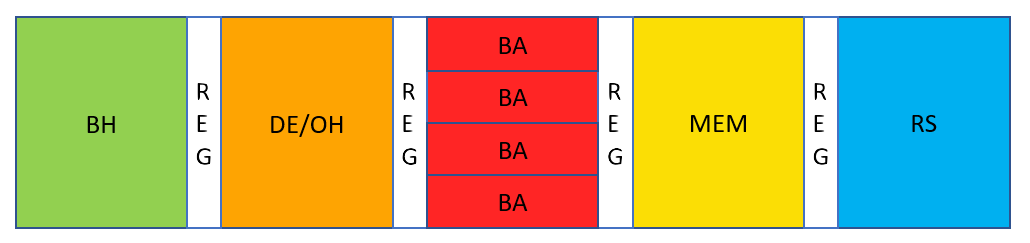
\includegraphics[scale=0.45]{Superskalare_Pipeline_mit_4_BA.png}
			\textbf{2-fach superskalare Pipeline mit 4 Recheneinheiten in der BA-Phase}\newline
			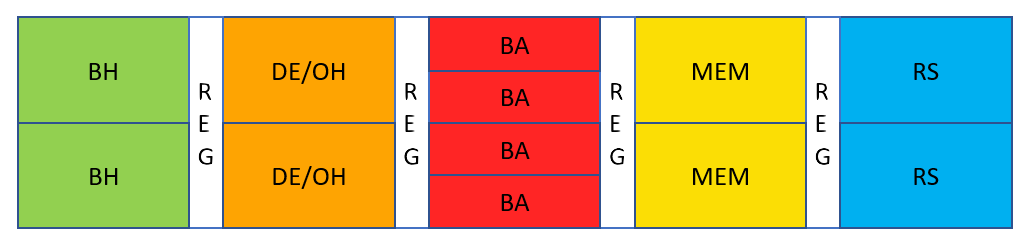
\includegraphics[scale=0.45]{2-fach_Superskalare_Pipeline_mit_4_BA.png}
		\end{center}
		\subsubsection{Dynamische Parallelisierung}
			Nicht alle Befehle eines sequentiellen Befehlsstrom können parallel ausgeführt werden. Datenhazards, also Datenabhängigkeiten zwischen Registern, sind ein Grund dafür. Bei Superskalarität wird deshalb spezielle Hardware eingefügt, die diese Abhängigkeiten erkennen und auflösen kann. \newline \newline
			Bei superskalaren Pipelines können auch Strukturhazards auftreten. Ein solcher tritt auf, wenn eine Recheneinheit (z.B. der Dividerer) benötigt wird, jedoch gerade noch durch eine andere Instruktion belegt ist. Auch für die Auflösung von Strukturhazards muss zusätzliche Hardware eingefügt werden, die die Belegung der Recheneinheiten überwacht und ggf. Befehle verzögert. \newline \newline
			Die Parallelisierung geschieht also zur Laufzeit durch die Hardware, was als dynamische Parallelisierung bezeichnet wird.
	\subsection{Very Long Instruction Word}
		Auch bei der Nutzung eines VLIW (Very Long Instruction Word) ist das Ziel die Beschleunigung der Abarbeitung von sequentiellen Programmen. Wie bei Superskalarität wird Parallelität auf Befehlsebene ausgenutzt. Im Gegensatz zur Ausführung bei Superskalarität werden die Befehle nicht dynamisch zur Laufzeit gruppiert, sondern statisch vom Compiler vor der Laufzeit. Dies wird auch als statische Parallelisierung bezeichnet \newline \newline
		Der Compiler fügt parallel ausführbare Instruktionen (ohne Datenabhängigkeiten!) zu einem Instruktionswort zusammen. Die maximal mögliche Anzahl ist dabei abhängig von der Länge des Instruktionswortes. Dieses durchläuft dann sequentiell die Pipeline: \newline
		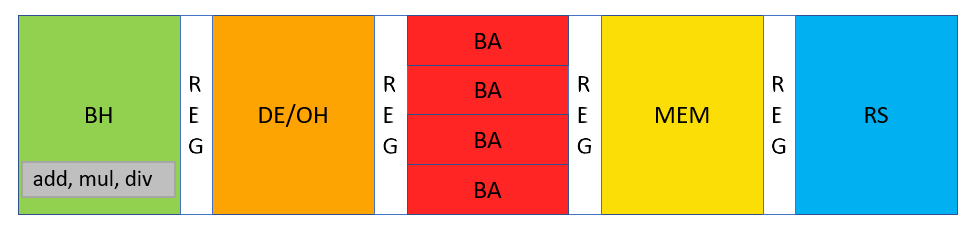
\includegraphics[scale=0.6]{VLIW_1.png}
		Wenn nicht genügend parallel ausführbare Operationen zur Verfügung stehen, muss der Compiler ein oder mehrere nop (no operation), also Platzhalter einfügen. Dadurch wird jedoch der Durchsatz verringert \newline
		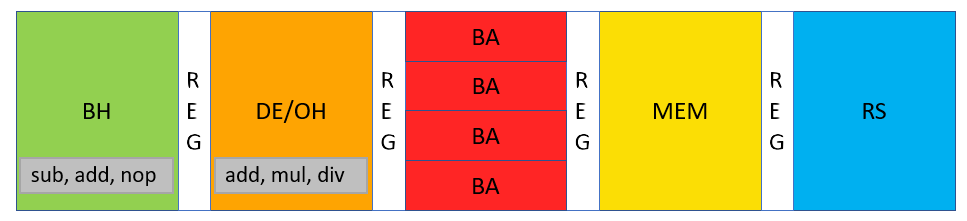
\includegraphics[scale=0.6]{VLIW_2.png} \newline
		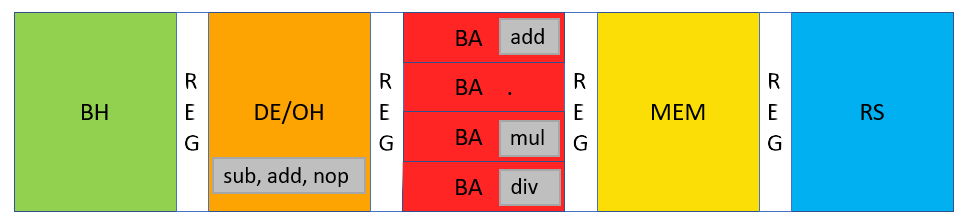
\includegraphics[scale=0.6]{VLIW_3.png}
	\section{Threadparallelismus}
	\section{Grafikkarten}
	\subsection{Grundlagen}
		\subsubsection{SIMD Prinzip}
			Single Instruction, Multiple Data. Dieses Prinzip beschreibt Instruktionsparallelismus, bei dem auf eine große Datenmenge parallel die gleiche Instruktion ausgeführt werden soll. Dies unterscheidet sich von dem dir bisher bekanntem SISD (Single Instruction, Single Data), bei dem in jeder "Programmzeile" eine beliebige Instruktion genannt wird, die dann wiederum auf 2 Eingabezahlen arbeitet \newline \newline
			SIMD Instruktionen zu unterstützen erfordert natürlich auch architekturelle Veränderungen am Rechner: Es müssen einerseits mehr homogene (d.h. gleichartige) Recheneinheiten (z.B. Addierer) hinzugefügt werden, die parallel arbeiten können. Manchmal wird stattdessen (um Platz zu sparen) auf andere Recheneinheiten (z.B. Multiplizierer) gänzlich verzichtet wird. Dadurch sind die Rechenoperationen, die nun nicht mehr verbaut sind, deutlich weniger performant umzusetzen (z.B. Multiplikation durch eine Vielzahl an Additionen). SIMD Rechner sind also kein grundsätzlicher Ersatz für normale SISD Rechner. \newline \newline
			Die Operanden-Hol-Phase und die Rückschreib-Phase benötigen außerdem (bestenfalls) eine breitere Speicheranbindung um mehr Daten pro Takt zu laden bzw. zurückzuschreiben. \newline
			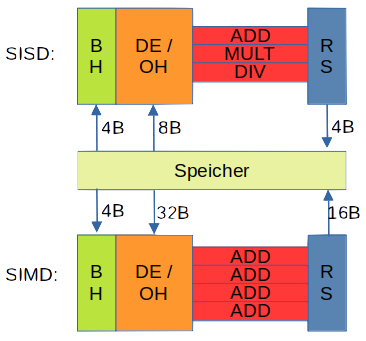
\includegraphics[scale=0.9]{simd.png}
			Bei Grafikkarten (GPUs) wird dieses architekturelle Prinzip auf die Spitze getrieben: Hier haben wir nur ein (oder ein paar wenige) Steuerwerke, die in jedem Takt nur einen (oder ein paar wenige) Operationen holen, und dann auf einer extrem großen Anzahl an Recheneinheiten (im Kontext von GPUs auch Shader genannt) diese Operation für große Datenmengen ausführen.
	\subsection{CUDA Modell}
		\subsubsection{GPU (Graphics Processing Unit)}
			Die Grafikkarte als Ganzes. Ein normaler Rechner besitzt in der Regel eine GPU (manchmal auch 2), oftmals als eigenes Gerät außerhalb der CPU. Günstige Rechner besitzen hingegen GPUs, die direkt mit in der CPU integriert sind (Integrated Graphics). Diese sind aber entsprechend sehr klein und leistungsschwach
		\subsubsection{Streaming Multiprocessor}
			Eine GPU besitzt ein oder mehrere Streaming Multiprocessors (SMs). Dies ist vergleichbar mit dem Konzept von Multicore bei CPUs: Jeder SM arbeitet unabhängig voneinander und kann auch tatsächlich verschiedene Instruktionen ausführen. SMs sind also relativ zueinander nicht SIMD
		\subsubsection{Shader}
			Ein Streaming Multiprocessor besteht aus einer Vielzahl an Shaders (typischerweise ca. 32). Diese Shader innerhalb eines SMs arbeiten nach dem SIMD Prinzip! Sie führen zeitgleich die exakt selbe Instruktion aus, auf unterschiedlichen Daten. Ein Shader beherrscht die absoluten Grundrechenoperationen, z.B. addieren und multiplizieren
		\subsubsection{Special Function Units}
			eder Streaming Multiprocessor besitzt neben den Shadern auch meistens noch 1-2 SFUs. Diese berechnen komplexere Dinge, wie z.B. Sinus oder Kosinus. Da wir davon aber nur sehr wenige haben, funktionieren sie nicht nach dem parallelen SIMD-Prinzip, sondern müssen sequentiell ausgeführt werden. Dies ist natürlich langsam - aber es ist immer noch schneller, als zu sagen, dass die GPU gar keinen Sinus/Kosinus kann und man jedes Mal diese Berechnung (die als Zwischenschritt in einem echten SIMD-Programm vorkommen könnte) an die CPU zu schicken \newline \newline
		\begin{center}
			\textbf{GPU mit 4 SMs, mit jeweils 12 Shadern und 2 FSUs} \newline
			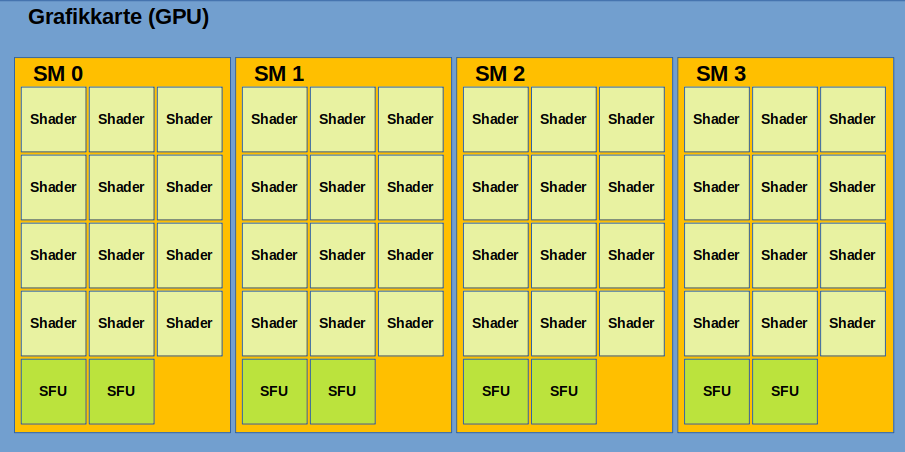
\includegraphics[scale=0.4]{gpu.png}
		\end{center}
	\subsection{CUDA Programmieren}
		Genau wie die Grafikkarten hierarchisch unterteilt ist (GPU -> Streaming Multiprocessor -> Shader) müssen beim CUDA-Modell auch Programmierer*innen ihr Problem unterteilen. Das Gesamtproblem kann man dabei als die gesamte Datenmenge verstehen, die verrechnet werden soll
		\subsubsection{Grid}
			Die gesamte Datenmenge, die von einer Grafikkarte (GPU) verrechnet werden soll, wird als "Grid" bezeichnet. Dies kann eindimensional (z.B. ein Vektor), zweidimensional (z.B. eine Matrix) oder dreidimensional (z.B. 3D Matrizen für 3D Computerspiele) sein
		\subsubsection{Block}
			Das Grid wird wiederum in Blöcke gleicher Größe unterteilt. Auch hier sind bis zu 3 Dimensionen möglich (sinnvollerweise identisch zur Griddimension). Ein Block wird von einem Streaming Multiprocessor bearbeitet	
		\subsubsection{Thread}
			Ein Block besteht wiederum aus mehreren Threads. Ein Thread ist in der Regel für nur ein Datenelement zuständig (theoretisch sind aber auch mehr möglich). Ein Thread wird von einem Shader ausgeführt \newline
		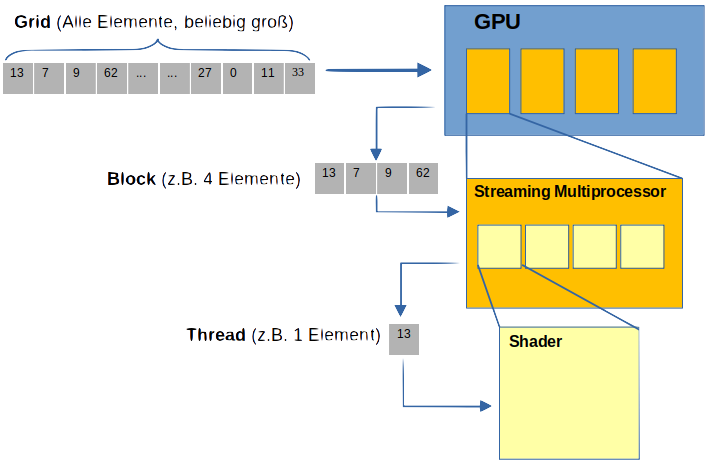
\includegraphics[scale=0.5]{cudamodell.png}
		\subsubsection{Code}
\begin{minted}{c}
__global__ void VectorAdd(float *vectorA, float *vectorB, int size){
	int index = blockIdx.x * blockDim.x * threadIdx.x;
	if (index < size)
		targetVector[index] = vectorA[index] * vectorB[index];	
	}
}
\end{minted}
			Die Funktion erhält als Funktionsargumente die Anfangsadressen der Vektoren  sowie die Gesamtgröße der Vektoren (damit wir nicht versehentlich Werte außerhalb der Vektoren betrachten \newline \newline
			In Zeile 3 bekommt jeder Shader mitgeteilt, für welches Element (bzw. welchen Index innerhalb des Vektors) er zuständig ist: Jeder Streaming Multiprocessor bekommt hierzu dynamisch vom GPU Scheduler einen sogenannten Block-Index (\verb|blockIdx|) zugewiesen, und jeder Shader darin bekommt dynamisch eine sogenannte Thread-ID (\verb|threadIdx|) zugewiesen. Da wir auch festgelegt haben, wie viele Threads es in einem Block gibt (\verb|blockDim|), kann jeder Shader sich dadurch seinen Vektorindex ausrechnen \newline \newline
			Anschließend wird geprüft, ob der Index überhaupt noch innerhalb des Vektors liegt. Wenn das der Fall ist, addieren wir die Werte der beiden Vektoren \verb|vectorA[index]| und \verb|vectorB[index]| zusammen und speichern es wiederum im Zielvektor \verb|targetVector[index]| 
		\subsubsection{Verzweigungen im CPU-Code}
			Bedingte Anweisungen, bei denen nur eine Teilmenge der Shader etwas rechnen soll, werden in der Regel so realisiert, dass durch die Bedingung die jeweils anderen Shader temporär "deaktiviert" werden. Am Ende der Verzweigung werden sie wieder "aktiviert".
			
	\section{Speicherverwaltung}
	\subsection{Virtuelle und physische Adressen}
		\subsubsection{Physische}
			Jedes Byte im physischen Arbeitsspeicher (d.h. im echten, vorhandenen Arbeitsspeicher) erhält in der Regel eine eigene Adresse, die sogenannte physische Adresse. Beim Starten des Rechners wird diese festgelegt und bleibt dann im laufenden Betrieb konstant. Anhand der physischen Adresse kann dann eindeutig bestimmt werden, in welcher Rank, Bank, Row und Column (Vgl. Tafelübung zu Arbeitsspeicher) sich ein bestimmtes Byte befindet
		\subsubsection{Virtuelle}
			Auf vielen Rechnern arbeiten Programme jedoch nicht mit den physischen, sondern mit sogenannten virtuellen Adressen. Würde ein Programm direkt mit physischen Adressen arbeiten, dann wären Konzepte wie Auslagerung (Swapping) oder Speicherschutz nicht mehr so einfach zu realisieren \newline \newline
			Virtuelle Adressen können vom Programm quasi frei gewählt werden. Mehrere Programme können auch die gleichen virtuellen Adressen verwenden, und dann damit aber unterschiedliche physische Adressen (und daher unterschiedliche Daten) meinen \newline \newline
			Virtuelle Adressen müssen, um physisch auf die Daten zugreifen zu können, in physische Adressen übersetzt werden. Das Festlegen von Übersetzungen verwaltet das Betriebssystem mittels sogenannter Übersetzungstabellen. Jeder Prozess bekommt eine eigene Übersetzungstabelle. Die Übersetzung - wenn eine festgelegt wurde - übernimmt in der Regel spezielle Hardware, die sogenannte Memory Management Unit (MMU). Diese liegt meistens direkt mit auf der CPU. Hierzu sagt das Betriebssystem der MMU, welcher Prozess gerade aktiv ist, indem die entsprechende Übersetzungstabelle als aktive Übersetzungstabelle festgelegt wird
		\subsubsection{Auslagerung (Swapping)}
			Bei der Auslagerung werden aktuell nicht benötigte Speicherbereiche vom Arbeitsspeicher auf die langsamere Festplatte verschoben. Dadurch schafft man neuen Platz im Arbeitsspeicher für aktive Prozesse, und hat somit quasi  mehr Arbeitsspeicher als eigentlich physisch vorhanden. Wenn auf die ausgelagerten Daten wieder zugegriffen werden soll, müssen diese erst wieder in den Arbeitsspeicher eingelagert und ggf. ein anderer Speicherbereich ausgelagert werden (tauschen => swapping). Dieser Vorgang ist langsam und daher ist es ratsamer, mehr physischen Arbeitsspeicher in den Rechner einzubauen, als den Arbeitsspeicher um die Festplatte zu erweitern
	\subsection{Paging}
		Bei Paging wird der Arbeitsspeicher in gleich große Bereiche (z.B. 4 KiB), sogenannte Pages, unterteilt. Pro Page, die verwendet werden soll, ist immer ein Eintrag in der Übersetzungstabelle (in diesem Kontext dann Page Table genannt) nötig \newline \newline
		Wenn ein Prozess nun Daten ablegen möchte, dann reserviert das Betriebssystem automatisch immer gleich eine ganze Page für diesen Prozess. Selbst wenn er nur 4 Byte ablegen möchte, bekäme er z.B. trotzdem direkt 4 KiB an Speicherbereich zugewiesen. Dies führt zu sogenannter interner Fragmentierung: Dieser Begriff bezeichnet ungenutzten Speicher innerhalb einer Page, der zu viel reserviert wurde \newline \newline
		\begin{center}
			\begin{tabular}{|c|c|c|}
				\hline
				Virt. Adresse & Phys. Adresse & Valid \\
				\hline
				... & ... & ... \\
				\hline 
				0x3CF & 0x4000 & 1 \\
				\hline
				0x3D0 & 0x5000 & 1 \\
				\hline 
				... & ... & ... \\
				\hline
				0x400 & 0x2000 & 1 \\
				\hline
				0x401 & 0x8000 & 1 \\
				\hline 
				... & ... & ... \\
				\hline
				0xF00 & 0xF000 & 1 \\
				\hline
				... & ... & ... \\
				\hline				
			\end{tabular}
		\end{center}
		\subsubsection{Byte-Offset}
			Bei einer 4KiB($2^{12}$ B) großen Page benötigt man 12 Bit um jedes Byte der Page zu adressieren. Demnach sind die letzten 3 Ziffern der virtuellen Adresse der Byte-Offset (0x 00 40 1\textbf{B 04}) und dieser muss anschließend auf die physische Adresse addiert werden (0x8\textbf{B 04})
	\subsection{Segmentierung}
		Bei der Segmentierung wird der Arbeitsspeicher - ähnlich wie bei Paging - in zusammenhängende Speicherbereiche aufgeteilt (sogenannte Segmente). Zusammenhängend bedeutet, dass Segmente nicht durchtrennt werden können; alle darin enthaltenen Bytes liegen sequentiell aufeinanderfolgend im Speicher \newline \newline
		Im Gegensatz zu Pages sind diese Segmente aber dynamisch groß, abhängig davon, wie viel Speicher der Prozess tatsächlich benötigt. Würde ein Prozess beispielsweise 3 KiB benötigen, dann würde er ein 3 KiB großes Segment bekommen \newline \newline
		Dies hat jedoch diverse Nachteile: 
		\begin{enumerate}
			\item Die Übersetzung (mittels der sogenannten Segment Tables) wird komplexer: Man muss bei jeder virtuellen Adresse prüfen, ob sie innerhalb eines dynamischen Bereichs liegt (definiert durch Startadresse + Größe des Segmentes). Dadurch ist das Segment nicht mehr berechenbar, sondern man muss es quasi suchen
			\item Externe Fragmentierung: Wenn Speicher reserviert wird, und wieder freigegeben wird, dann können ungleich große Lücken zwischen Segmenten entstehen. Diese Lücken sind dann gegebenenfalls in der Summe groß genug für ein neues Segment, aber jedes einzelne ist nicht ausreichend groß. Da Segmente zusammenhängend sein müssen, kann man es nicht auf mehrere Lücken aufteilen
			\item Verbunden damit ist auch eine allgemein komplexe Suche nach freiem Speicher. Da man nach möglichst ideal großen Lücken suchen muss, kann das Speicherreservieren länger dauern. Bei Paging hingegen sind ohnehin alle Pages gleich groß, also würde man hier die erste freie immer nehmen
		\end{enumerate}
	\subsection{Translation-Lookaside-Buffer (TLB)}
		 Der TLB ist ein Spezialcache, der sich die letzten ca. 4 - 32 Adressübersetzungen merkt. Bei einer Adressübersetzung wird damit zuerst geprüft, ob die physische Adresse vielleicht bereits bekannt ist; und ansonsten wird die Übersetzung eben manuell über die Übersetzungstabellen durchgeführt und sich das Resultat davon gemerkt
\end{document}